\documentclass[12pt,a4paper,onecolumn]{article}
\usepackage{paralist}
\usepackage{indentfirst}
\usepackage[numbers,sort&compress]{natbib}
\usepackage[left=1.5cm,right=1.5cm,top=1.5cm,bottom=1.5cm]{geometry} %页边距包
\usepackage{amsmath}
\usepackage{flushend,cuted}
\usepackage{caption}
\usepackage{subcaption}
\usepackage{ctex}
\usepackage{pifont}
\usepackage{hyperref}
\usepackage{float} %控制图像固定
\usepackage{listings} %代码
\usepackage{color}
\definecolor{mygreen}{rgb}{0,0.6,0}
\definecolor{mygray}{rgb}{0.5,0.5,0.5}
\definecolor{mymauve}{rgb}{0.58,0,0.82}
\lstset{ %
	backgroundcolor=\color{white},   % choose the background color; you must add \usepackage{color} or \usepackage{xcolor}
	basicstyle=\footnotesize,        % the size of the fonts that are used for the code
	breakatwhitespace=false,         % sets if automatic breaks should only happen at whitespace
	breaklines=true,                 % sets automatic line breaking
	captionpos=b,                    % sets the caption-position to bottom
	commentstyle=\color{mygreen},    % comment style
	deletekeywords={...},            % if you want to delete keywords from the given language
	escapeinside={\%*}{*)},          % if you want to add LaTeX within your code
	extendedchars=true,              % lets you use non-ASCII characters; for 8-bits encodings only, does not work with UTF-8
	%frame=single,	                   % adds a frame around the code
	keepspaces=true,                 % keeps spaces in text, useful for keeping indentation of code (possibly needs columns=flexible)
	keywordstyle=\color{blue},       % keyword style
	language=python,                 % the language of the code
	otherkeywords={*,...},           % if you want to add more keywords to the set
	numbers=left,                    % where to put the line-numbers; possible values are (none, left, right)
	numbersep=5pt,                   % how far the line-numbers are from the code
	numberstyle=\tiny\color{mygray}, % the style that is used for the line-numbers
	rulecolor=\color{black},         % if not set, the frame-color may be changed on line-breaks within not-black text (e.g. comments (green here))
	showspaces=false,                % show spaces everywhere adding particular underscores; it overrides 'showstringspaces'
	showstringspaces=false,          % underline spaces within strings only
	showtabs=false,                  % show tabs within strings adding particular underscores
	stepnumber=1,                    % the step between two line-numbers. If it's 1, each line will be numbered
	stringstyle=\color{mymauve},     % string literal style
	tabsize=2,	                   % sets default tabsize to 2 spaces
	%title=\lstname                   % show the filename of files included with \lstinputlisting; also try caption instead of title
}
\renewcommand\refname{参考文献}
\newcommand{\upcite}[1]{\textsuperscript{\textsuperscript{\cite{#1}}}}
\linespread{1.5}
\hypersetup{
  colorlinks,
  linkcolor=green,
  urlcolor=blue
}
\setCJKfamilyfont{zhsong}{SimSun}
\newcommand{\fs}{\CJKfamily{zhfs}}

\title{使用快速傅立叶变换进行信号分离}
\date{}
\author{黎思言}

\begin{document}
\captionsetup[figure]{name={图}}
\captionsetup[table]{name={表}}
\renewcommand{\abstractname}{}
\maketitle

\begin{abstract}
	傅里叶变换(Fourier transform)是一种线性的积分变换。基本思想首先由法国学者傅里叶系统地提出。他认为现实世界中任何周期函数,都可以看作是不同振幅,不同相位正弦波的叠加。根据函数的形式不同,可以把傅立叶变换分为四种类别:1、非周期性连续信号——傅立叶变换(Fourier Transform)2、周期性连续信号——傅立叶级数(Fourier Series)3、非周期性离散信号——离散时域傅立叶变换(Discrete Time Fourier Transform)4、周期性离散信号——离散傅立叶变换(Discrete Fourier Transform)。离散傅立叶变换(DFT)可以将一条周期性离散信号转换成多条正弦信号或者余弦信号的累加。快速傅立叶变换(FFT)是一种求解离散傅立叶变换(DFT)的快速算法。在本文中,我就使用了快速傅立叶变换,求解离散信号分离问题。
\end{abstract}

\section{计算步骤}

(1)假设我们拥有一条长度为$N$的观测$y$。我们将每一个观测点表示成$y[i]$($i$的取值范围是1到$N$)。$y$此时在时域空间中是一个$1\times N$的向量。
$$y=[y_1,y_2,...,y_N]$$

(2)使用快速傅立叶变换(FFT)将$y$投影到频域空间中。投影的结果是一个长度为$N/2+1$的复数$Y$。复数的实部表示为$ReY[k]$,虚部表示为$ImY[k]$($k$的取值是0到$N/2$)。\footnote{在python的FFT算法中,实际上输出了长度为N的复数,但是这个复数前半部分和后半部分是完全对称的。}
$$y=[y_1,...,y_N]\xrightarrow{FFT} Y=[ReY_0+iImY_0,...,ReY_{N/2}+iImY_{N/2}]$$

需要区分的是,$k$表示的含义和$i$表示的含义是完全不同的。$i$可以理解为时域空间中的一个时间点,$y[i]$可以理解为在第$i$个时间点上,我们观察到的振幅的大小。$k$可以理解为频域空间中的某一个频率取值,$Y[k]$可以理解为在第$k$个频率取值上,我们观察到的特征。

为什么$Y$的长度是$N/2+1$?这是因为只有$N$个观测点,所以我们最多只能用$N/2+1$个频率来拟合。

FFT究竟是如何投影过去的?这个问题超级复杂,不是我们关注的重点,只要知道它能用就行。

(3)使用离散傅立叶变换的逆变换,将频域信息投影到时域。
$$y_i=\sum_{k=1}^{N/2}(\frac{ReY[k]}{N/2}cos(2\pi ki/N)+(-\frac{ImY[k]}{N/2})sin(2\pi ki/N))$$

如何直观的解释上式呢?我们在时域空间中观察到某一个时间点$i$的振幅$y_i$,可以表示成在频域空间中所有频率$k$下的特征和正余弦函数的线性组合的累加。

由上式还易知,$Y$的模就是时域空间中的振幅。依据这一条信息,我们就可以舍弃那些模比较小的,留下那些模比较大的复数来近似拟合时域空间。如此一来,一条复杂的,特征不明的时域空间的曲线就被分解成了多条正余弦曲线。

\section{python实现方法}

\begin{figure}[H]
	\centering
	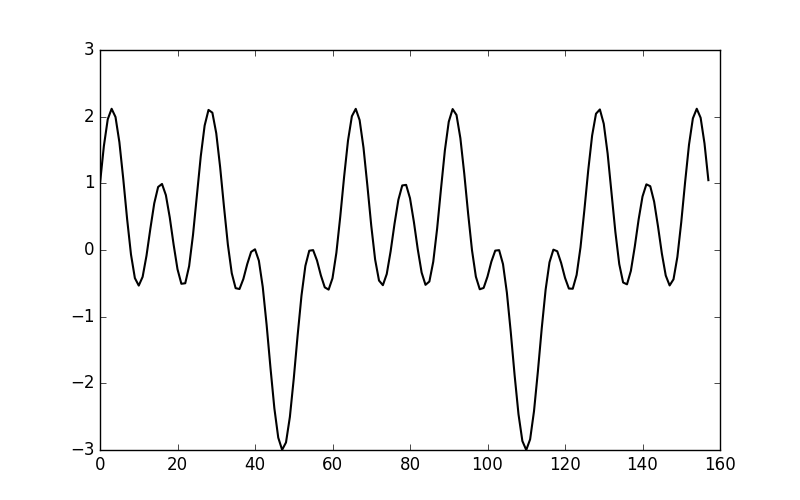
\includegraphics[width=400pt]{fig0.png}
	\caption{原始信号}
\end{figure}

(1)读入原始信号并观察信号特征。图1是我们的原始信号。可以发现这是一条周期性离散信号,应该用离散傅立叶变换求解。读入数据并绘图的python代码如下所示。

\begin{lstlisting}
	dat=[s for s in open("Data.txt").readlines()]
	dat=[s.strip() for s in dat]
	for i in range(len(dat)):
	    if dat[i]=="Data_y:":
	        print i

	y=[float(s) for s in dat[162:]]
	n=len(y)

	plt.figure(figsize=(8,5))
	plt.plot(range(n),y,lw=1.5,color="black")
	plt.xlim(0,160)
	plt.ylim(-3,3)
	plt.savefig("fig0.png")
\end{lstlisting}

(2)使用numpy.fft.fft函数将时域信号转换成频域信号。python代码如下所示。

\begin{lstlisting}
	y_fft = np.fft.fft(y)
	y_fft=y_fft[:(n/2+1)]
	real=y_fft.real/(n/2)
	imag=-y_fft.imag/(n/2)
\end{lstlisting}

(3)使用所有的频率特征来还原信号。公式:$$\hat{y_i}=\sum_{k=1}^{N/2}(\frac{ReY[k]}{N/2}cos(2\pi ki/N)+(-\frac{ImY[k]}{N/2})sin(2\pi ki/N))$$

\begin{figure}[H]
	\centering
	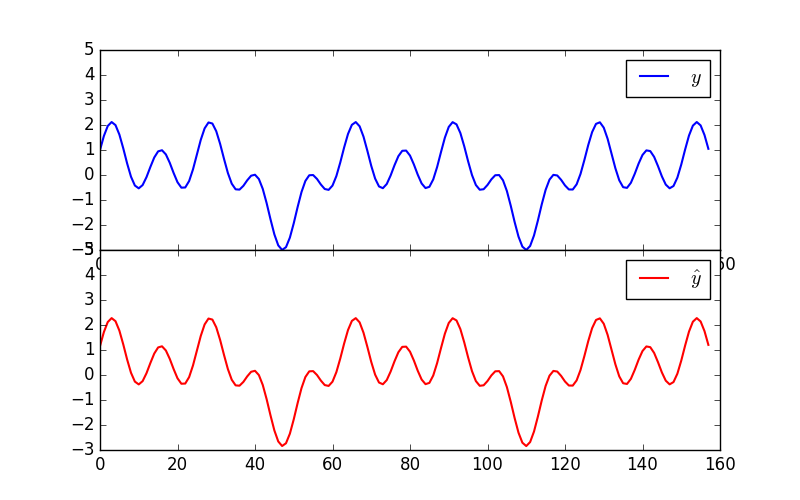
\includegraphics[width=400pt]{fig1.png}
	\caption{使用所有的特征还原信号}
\end{figure}

还原结果如图2所示,蓝色的线条表示原始数据信号,红色线条表示使用FFT分解过后的所有频域信号还原的时域信号。这两条信号几乎是完全一样的。python代码如下所示。

\begin{lstlisting}
	y_hat=[]
	for i in range(n):
	    tmp=np.sum(real[k]*np.cos(2*np.pi*k*i/n)+imag[k]*np.sin(2*np.pi*k*i/n) for k in range(n/2+1))
	    y_hat.append(tmp)

	plt.figure(figsize=(8,5))
	plt.subplots_adjust(hspace=0)
	plt.subplot(211)
	plt.plot(range(n),y,lw=1.5,color="blue",label="$y$")
	plt.xlim(0,160)
	plt.ylim(-3,5)
	plt.legend()
	plt.subplot(212)
	plt.plot(range(n),y_hat,lw=1.5,color="red",label="$\hat{y}$")
	plt.xlim(0,160)
	plt.ylim(-3,5)
	plt.legend()
	plt.savefig("fig1.png")
\end{lstlisting}

(4)找到频域空间中振幅较大的信号。频域空间的振幅是复数$Y$的模,频率是$Y$的序号。我用$Y$的序号为横轴,$Y$的模为纵轴绘图(图3)可知,频域空间中振幅最大的三条信号的频率分别是$k=5,k=2,k=13$。python代码如下所示。

\begin{figure}[H]
	\centering
	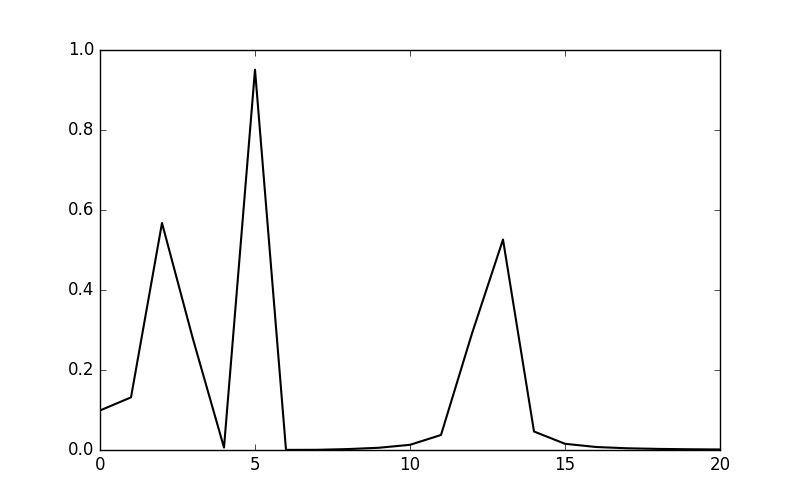
\includegraphics[width=400pt]{fig2.png}
	\caption{频谱}
\end{figure}

\begin{lstlisting}
	mod=[]
	for i in range(len(real)):
	    tmp=real[i]**2+imag[i]**2
	    mod.append(tmp)

	plt.figure(figsize=(8,5))
	plt.plot(range(len(mod)),mod,lw=1.5,color="black",label="$mod$")
	plt.xlim(0,20)
	plt.savefig("fig2.png")

	top3=np.argsort(-np.array(mod))[:3]
\end{lstlisting}

(5)使用频率为$k=5,k=2,k=13$的三条信号还原信号。
\begin{align*}
	\hat{y^{(1)}_i} &=\frac{ReY[5]}{N/2}cos(2\pi 5i/N)+(-\frac{ImY[5]}{N/2})sin(2\pi 5i/N) \\
	              &=0.97cos(0.063\pi i)-0.089sin(0.063\pi i)
\end{align*}
\begin{align*}
	\hat{y^{(2)}_i} &=\frac{ReY[2]}{N/2}cos(2\pi 2i/N)+(-\frac{ImY[2]}{N/2})sin(2\pi 2i/N) \\
	              &=0.753cos(0.025\pi i)-0.028sin(0.025\pi i)
\end{align*}
\begin{align*}
	\hat{y^{(3)}_i} &=\frac{ReY[13]}{N/2}cos(2\pi 13i/N)+(-\frac{ImY[13]}{N/2})sin(2\pi 13i/N) \\
	              &=-0.705cos(0.165\pi i)+0.171sin(0.165\pi i)
\end{align*}

将三条信号求和并化简,得到以下表达式(正弦形式):
\begin{align*}
	\hat{y_i} &=\hat{y^{(1)}_i}+\hat{y^{(2)}_i}+\hat{y^{(3)}_i} \\
	          &=0.975sin(0.063\pi i-0.092)+0.753sin(0.025\pi i-0.037)+\\
	          &\quad 0.073sin(0.165\pi i-0.238)
\end{align*}

\begin{figure}[H]
	\centering
	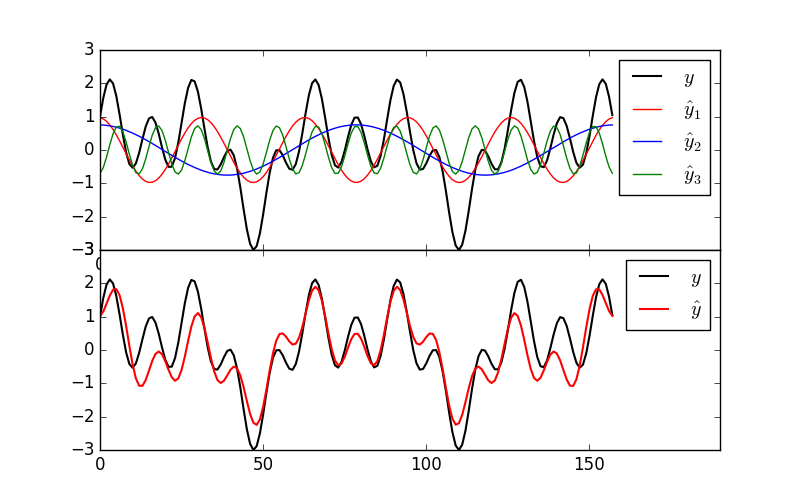
\includegraphics[width=400pt]{fig3.png}
	\caption{使用三条模最大的信号还原信号}
\end{figure}

还原结果如图4所示,上图黑色线条表示原信号,红蓝绿三色线条表示频域空间中模最大的信号在时域空间中的图像。下图黑色线条表示原信号,红色线条表示上述三条信号的合成信号。可知合成信号已经很好的拟合了原始信号。python代码如下所示。

\begin{lstlisting}
	def myfun(k):
	    curve=[real[k]*np.cos(2*np.pi*k*i/n)+imag[k]*np.sin(2*np.pi*k*i/n) for i in range(n)]
	    return curve

	[curve1,curve2,curve3]=[myfun(k) for k in top3]
	curve=[curve1[i]+curve2[i]+curve3[i] for i in range(n)]
	plt.figure(figsize=(8,5))
	plt.subplots_adjust(hspace=0)
	plt.subplot(211)
	plt.plot(range(n),y,lw=1.5,color="black",label="$y$")
	plt.plot(range(n),curve1,lw=1,color="red",label="$\hat{y}_1$")
	plt.plot(range(n),curve2,lw=1,color="blue",label="$\hat{y}_2$")
	plt.plot(range(n),curve3,lw=1,color="green",label="$\hat{y}_3$")
	plt.xlim(0,190)
	plt.ylim(-3,3)
	plt.legend()
	plt.subplot(212)
	plt.plot(range(n),y,lw=1.5,color="black",label="$y$")
	plt.plot(range(n),curve,lw=1.5,color="red",label="$\hat{y}$")
	plt.xlim(0,190)
	plt.ylim(-3,3)
	plt.legend()
	plt.savefig("fig3.png")
\end{lstlisting}

\end{document}
